%************VERSUCHSANORDNUNG*************
\chapter{Experimental Setup}
\label{sec:versuchsandordnung}
The experimental work done in this thesis primarily utilized a Low-Temperature Scanning Tunneling Microscope setup (LT-STM).
This STM is composed of two distinct compartments, the preparation chamber (PC) and the measurement chamber (MC).
The sample is inserted through an airlock into the preparation chamber.
In the whole system Ultra High Vacuum (UHV) at about 10$^{-11}$ - 10$^{-10}$ mbar is maintained, which is archieved by four individual pumps.
The base Vacuum is achieved with the turbomolecular pump and the scroll pump through the airlock.
Additionally, there is a titanium sublimation pump and an ion pump in the preparation chamber.

\monofig{width=\textwidth}{Experimental_Setup/STM_Picture_1_edited.pdf}{
    The experimental setup used, 
    A: cryostat filled with Liquid Nitrogen,
    B: measurment-chamber with spring suspended STM,
    C: sputter-gun,
    D: metal-evaporater,
    E: molecule-evaporater,
    F: preparation-chamber with sample manipulator,
    G: LEED system,
    H: Electronic used to monitor the function of the STM}{fig:stm_uni_kf}
%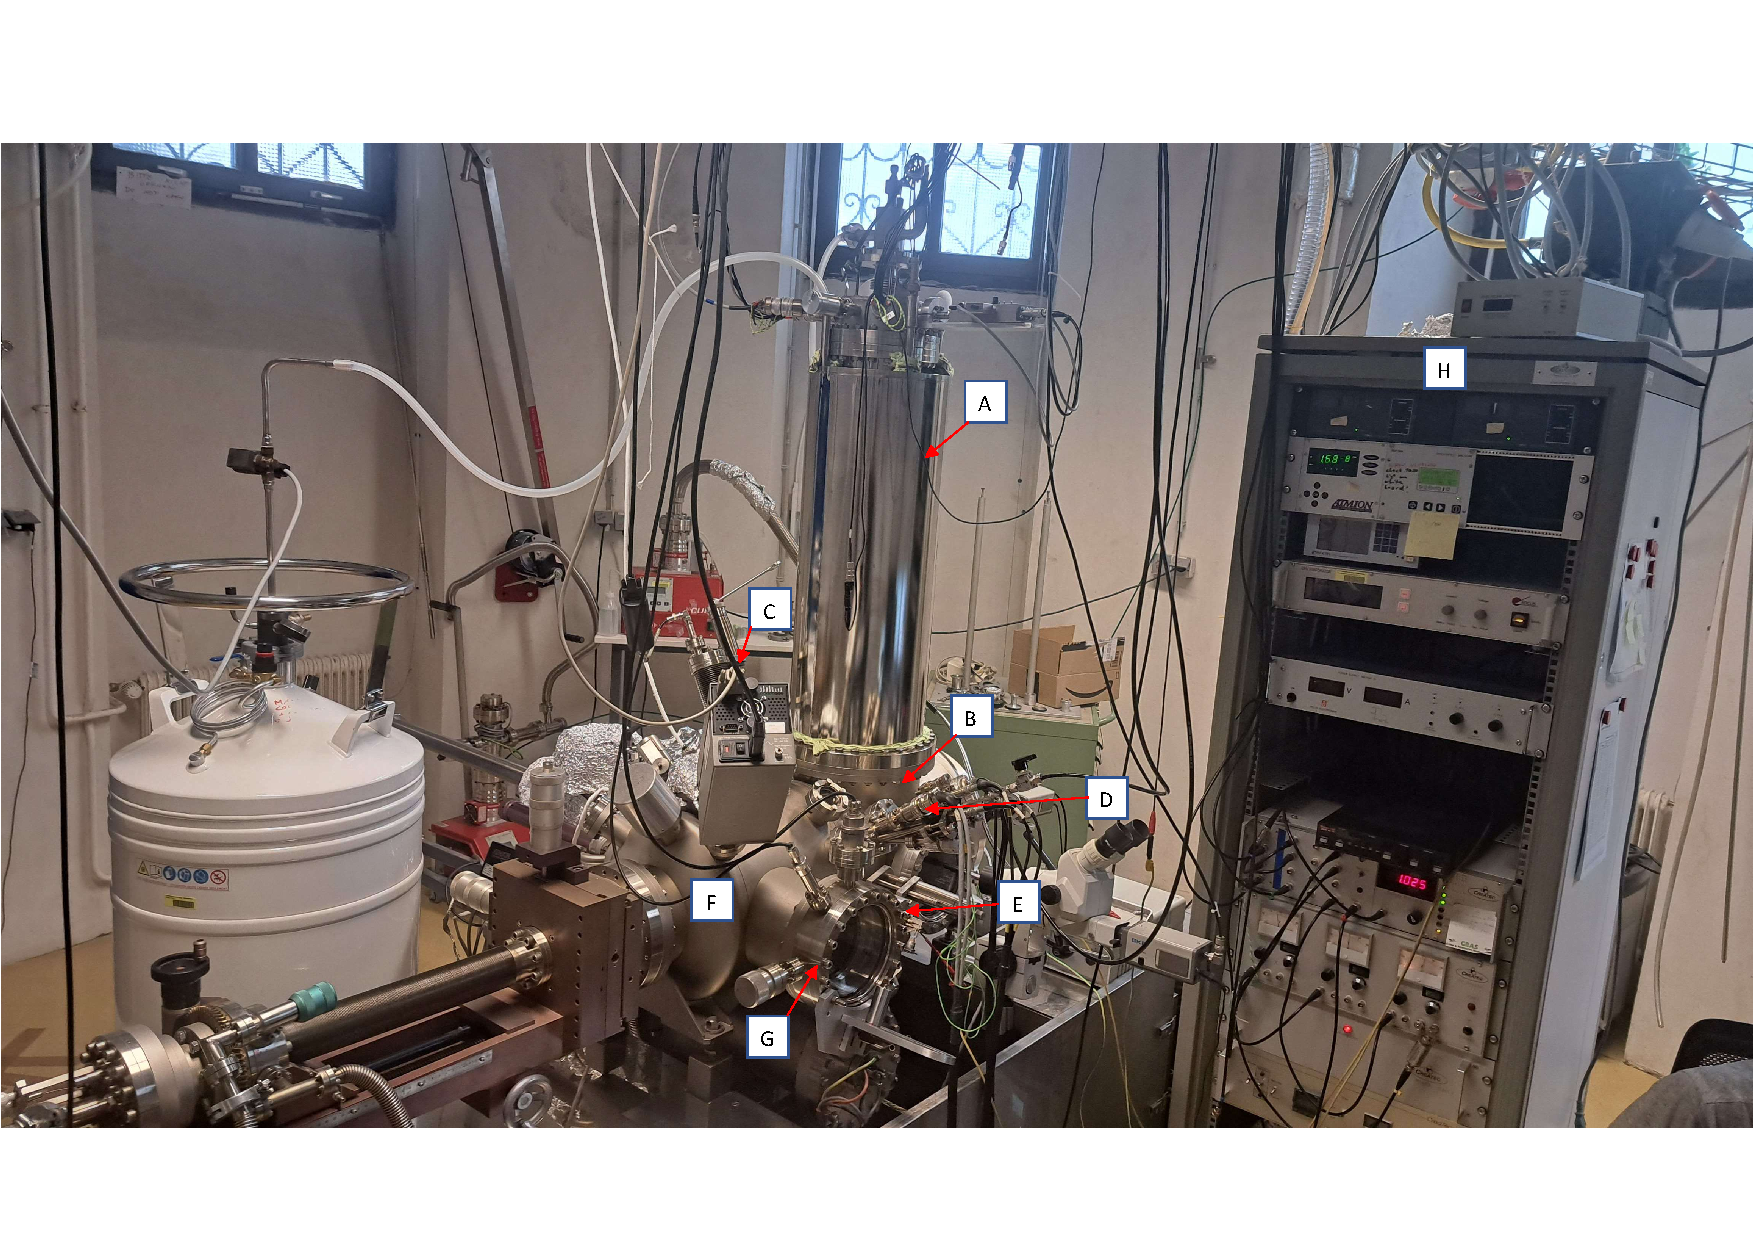
\includegraphics[width=0.9\textwidth]{Experimental_Setup/STM_Picture_1_edited.pdf}

The manipulator can be moved in each direction and rotated around its z-axis.
It is also used to insert the Sample-holder into the STM.
The PC contains a LEED system, which fluorescent screen can be extended. 
Additionally the PC has a metal-evaporator (E-beam evaporator) and a organic-molecule evaporator  (triple Knudsen cell) which are used for sample preparation.
The sample is mounted onto the previously mentioned Sample-holder with a Heatwaves Labs Inc. button sample heater with a resistive heating range of 20 K - 900 K.
The sample can also be cooled using LN2 or LHe through a built-in pipe system in the manipulator arm.
A Quartz-Crystal Microbalance (QCM) with sub Angstöm precision is used to monitor the deposition rate.
To clean the sample, an Argon sputter gun is employed, which utilizes an electric field to ionize and accelerate argon gas.
The MC consists of a LT-STM which is mounted to a two-shell cryostat, and surrounded by two radiation shields to achieve temperatures as low as 7 K, when cooled with Liquid Helium.
In this thesis the cryostat chamber was filled with LN2 which means it was operated at 75 K.
The primary measuring unit (STM) is vibrationally damped using a coupled spring system.

\section{Sample Preparation}
\subsection{Silver (Ag)}
\noindent The Substrate used in this thesis is a Silver Ag(100) single crystal.  
Silver naturally crystallizes into a face centered curbic (fcc) structure with a lattice constant of a = 4.079 \AA. \cite{PhysRev.25.753}
The single crystal is cut along the (100) plane giving it a square surface lattice along the [011] and [01$\bar{1}$] Direction, with a neares neighbor distance 2.884 \AA.
To ensure that the surface is clean, multiple cycles of Argon-Ion Sputtering with consequent annealing were performed. 
The first preparation was done with 3x Sputtering for 5 min each and annealing at 500 C° for 3-5 min.
Later a longer sputtering time of 20 min proved more effective.  
Prior to the metal or organic adsorbtion the substate is cooled to room temperature.
\monofig{width=0.7\textwidth}{\\Experimental_Setup\\Silver.PNG}{(a) Crystal lattice structure of an fcc Ag single crystal sectioned along the (100) plane. (b) Top View with the depicted nearest neighbor distance of 2.884 \AA \cite{hollerercharge}}{fig:silver_lattice}
\subsection{Magnesium Oxide (MgO)}
The crystal structure of MgO is fcc with a lattice constant of a = 4.22 \AA  \cite{guilliatt1969lattice}, which makes it only 3.4 \% larger than Ag.
This allows for the formation of ultrathin MgO(100) films on Ag(100). with relativly large, defect free terrases. 
The preparation on Ag(100) is done using a E-beam evaporator, in which a filament is heated, causing it to emit electrons.
These electrons are than accelerated using a high voltage (250-300V) onto the Magnesium crucible.
The product of the emission current and acceleration voltage is the heating power.
To ensure a monolayer the deposition rate is measured using a Quarz-Crystal Microbalance (QCM).
A deposition rate of 0.5 \AA/min is established.
Magnesium is than deposited onto the Ag(100) substrate,which is heated to 300 °C, while Oxygen O$_2$ is being fed into the Preparation Chamber (10$^{-6}$ mbar).
After the film is deposited, the sample is being slowly cooled at a cooling rate of 5 K/min to room temperature.
This ensures larger terrases as MgO is known to break into small islands if cooled to fast. \cite{pal2014morphology}
\monofig{width=0.7\textwidth}{\\Experimental_Setup\\MgO.PNG}{(d) Crystal lattice structure of 2 ML MgO(100) on Ag(100) sectioned at the (100) plane, (e) Top View with the depicted nearest neighbor distance of $\frac{a}{\sqrt{2}}$ \cite{hollerercharge}}{fig:MgO_lattice}
\newpage
\subsection{Pentacenequinone}
Pentacenes are a organic molecule group with five linearly organised benzene rings, which share two neighboring carbon atoms.
The carbon atoms are sp$^2$ hybridised, which gives it a hexagonal structure in which the single- and double-bond is alternating.
The $\pi$ orbitals extend out of the molecular plane.
These overlapping  $\pi$ orbitals result in delocalized electrons, which makes it a conjugated $\pi$-bond system. \\
\begin{wrapfigure}{r}{0.5\textwidth}
    \centering
    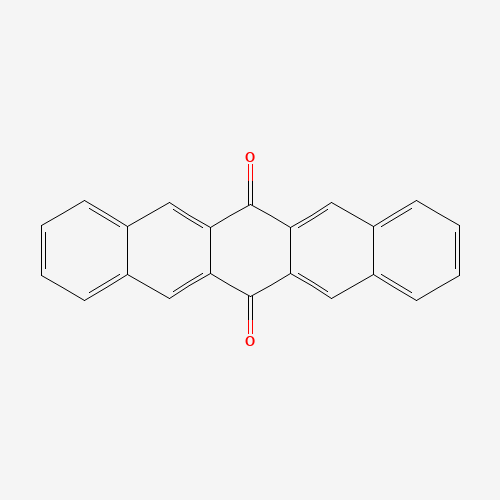
\includegraphics[width=0.49\textwidth]{graphics/6,13-Pentacenequinone.png}
    \caption{The structure of Pentacenequinone  \cite{pentacenequinone}}
    \label{fig:penta}
\end{wrapfigure}
\noindent Quinone refers to the replacement of two hydrogen atoms with two oxygen atoms in a benzene ring %[\cite{NIAZ2020749}].
The two carbonyl groups (C=O) in this adsorbate are located on the central ring.
Pentacene is an organic p-type semiconductor, which is used in the domain of organic electronics.
It is remarkably stable and has a high charge mobility for an organic molecule of 2.2 cm$^2$ V$^{-1}$ s$^{-1}$. \cite{MOTA2018511}
Pentacenequinone exibits similar properties and is used as a precursor for the synthesis of pentacene. \\

\newpage
\subsection{2-Hydrogen Phthalocyanine}
Phthalocyanines are a group of organic molecules that are structurally related to porphyrins and are mostly used as a blue pigment. \cite{thomas1990phthalocyanine}
Other applications are nonlinear optical materials, enzyme-like catalysts, liquid crystals, sensitizers, photovoltaic cells or even as photodynamic reagents for cancer therapy. \cite{wang2012structures}
They are characterized by a symmetric macrocyclic structure of four isoindole units [(C$_6$H$_4$)C$_2$N], which consists of a pyrole unit fused with a benzene ring. 
The isoindole units are linked by four nitrogen atoms (aza-bridges) forming a conjugated ring.
This allows delocalization of the $\pi$ electrons across the macrocycle.



\begin{wrapfigure}{l}{0.5\textwidth}
    \centering
    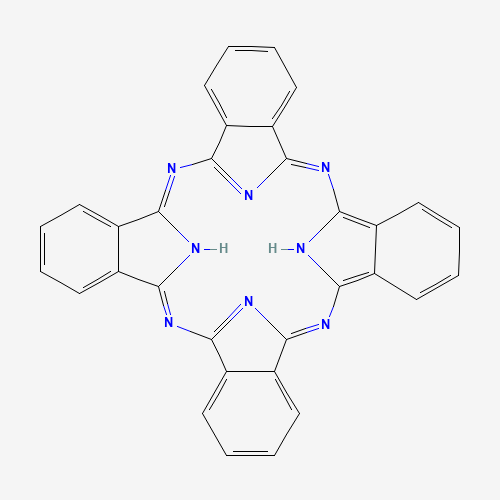
\includegraphics[width=0.49\textwidth]{graphics/Phthalocyanine.png}
    \caption{The structure of 2-H Phthalocyanine \cite{phthalacyanine}}
    \label{fig:phtalo}
\end{wrapfigure}

There are more than 70 variations of phthalocyanines, with they key difference in the substitution of different elements or transition metals (e.g. Cu$^{2+}$ and Ni$^{2+}$) in the middle of the molecule \cite{thomas1990phthalocyanine}.
The physical properties can be altered by the choice of different metal ions, like the adsorbtion characteristics or the geometry of the molecule itself. 
In this thesis, 2-Hydrogen Phthalocyanine is studied, which harbors, two hydrogen Atoms in the middle of the Macrocycle attached to two opposing pyrole units.
Generally Phthalocyanines are remarkably chemically and thermally stable \cite{thomas1990phthalocyanine}.
This can be attributed to its planar geometry and conjugated macrocycle.
Phthalocyanines are used as as dye for textiles and as inks because they strongly absorb light in the visable range especially in 620 - 750 nm regime, which makes them appear dark green-blue. 
They are also known for their optical, electronic and photo-electronic properties, all of which make them a promising chemiresistor sensor.
Because of the semiconducting properties of phthalocyanins, their capability as a transistor, its use as liquid crystal display or its solar-cell applications are investigated. 